\documentclass[sigconf]{acmart} %Recommended doc class from Lins;
\acmConference[Robo-Maze Blast Project]{
	University for Applied Sciences Hamburg\\
	Department of Computer Science}{2025}{Hamburg, Germany}
% Remove conference-specific formatting
\settopmatter{printacmref=false}  % Disables "ACM Reference Format"
\setcopyright{none}               % Removes copyright notice

\acmBooktitle{}                   % Removes booktitle
\acmDOI{}                         % Removes DOI
\renewcommand{\acmPrice}{}        % Removes price
% Language setting
% Replace `english' with e.g. `spanish' to change the document language
\usepackage[english]{babel}
\usepackage[ruled,vlined]{algorithm2e}
% Set page size and margins
% Replace `letterpaper' with `a4paper' for UK/EU standard size

% Useful packages
\usepackage{amsmath}
\usepackage{graphicx}
\title{Robo-maze Blast Report}
\author{Dogà Sara}
\author{Widmann Lukas}
\author{Askar Sami}

\begin{abstract}
Bomberman + Evolutionary algorithmens + Tournament Arc goes brr 
\end{abstract}

\begin{document}
\maketitle



\section{Introduction}

\subsection{The game}
\href{https://codeberg.org/chrlns/robo-maze-blast.git}{Robo Maze Blast}, created in 2008 by Kai Ritterbusch and Christian Lins, is a clone of the Bomberman game. Also known as Dynablaster, it is a strategy maze-based video game franchise originally developed by Hudson Soft in 1985.

The general goal of Bomberman is to complete the levels by strategically placing bombs in order to kill enemies and destroy blocks. Some blocks in the path can be destroyed by placing bombs near it, and as the bombs detonate, they will create a burst of vertical and horizontal lines of flames. Except for indestructible blocks, contact with the blast will destroy anything on the screen.

\subsection{Our Goal}
The aim of our project is to explore the efficiency of different Genetic Algorithms to develop 3 agents with strategic competence in the Robo Maze Blast scope, and to compare them by making the agents fight against each other and observe which agent outlives the others more frequently.

\section{Background}
\subsection{Genetic Algorithms}
Genetic Algorithms (GA) are optimization algorithms inspired by the process of natural selection and biological evolution. They are widely used to solve complex optimization and search problems in various domains. 
One of those domains is the gaming side as in this paper. 
\begin{figure}
      \centering
      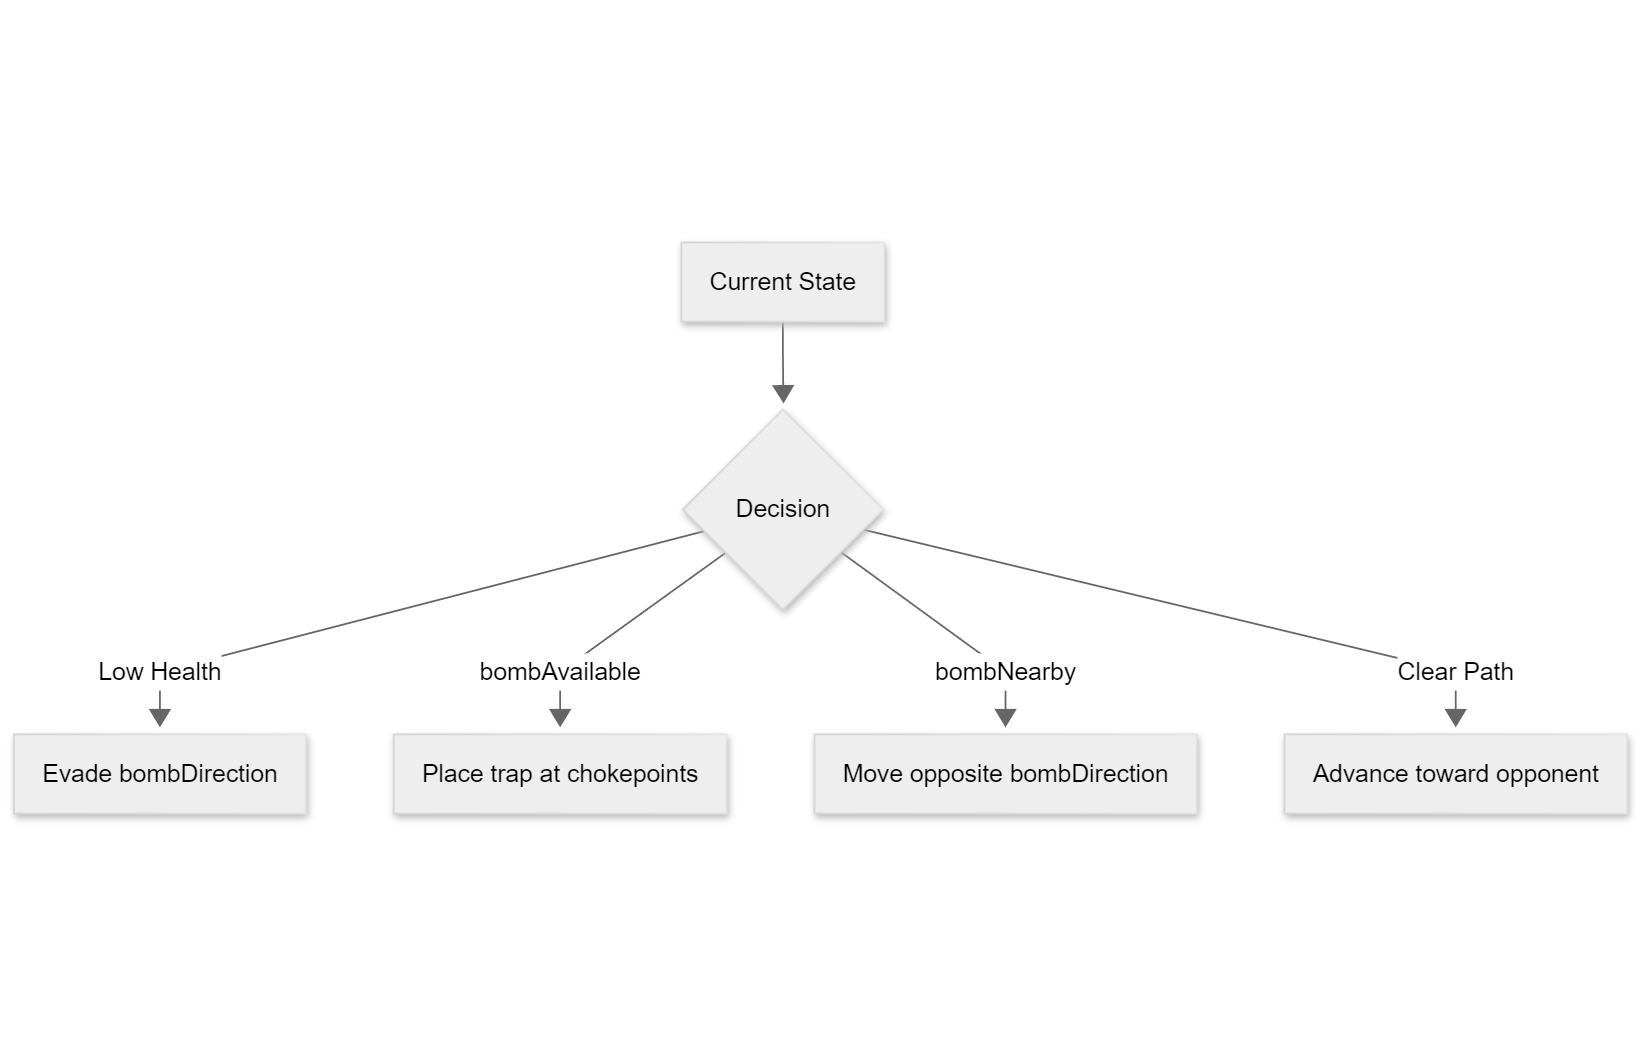
\includegraphics[width = 1\linewidth]{pictures/possibleActionsPlayer.png}
      \caption{\label{fig:possibleActionsPlayer}A diagram on the possible actions of a player}
      \end{figure}
Due to constrained optimization (e.g., state/action of the game), Genetic Algorithms are a perfect choice for this task \cite{popescu2025}: 
\textit{``Genetic Algorithms (GAs) were selected for their ability to handle complex combinatorial optimization problems [...] and to encode domain-specific constraints"} (Section 1).

The core steps of a typical genetic algorithm can be described as follows:
\begin{itemize}
    \item \textbf{Population Base}: Initialize a population from valid chromosomes, i.e. a set of strings that encodes any possible solution. Usually, the initial population is chosen randomly.
    \item \textbf{Evaluation}: Each population solution is evaluated on the basis of a predetermined fitness function.
    \item \textbf{Selection}: Reproductive opportunities are allocated to the chromosomes that represent a better solution to the target problem, and such solutions are selected to form a 'mating pool' for the next generation.
    \item \textbf{Crossover and Mutation}: The selected individuals are then combined to produce offspring by exchanging genetic material. Sometimes small changes can happen in the genetic material, such as bit flips. All of this ensures good exploration of the solution space and diversity.
    
\end{itemize}
These steps are repeated for a number of times until an ending criterion is reached.

\begin{figure}
\centering
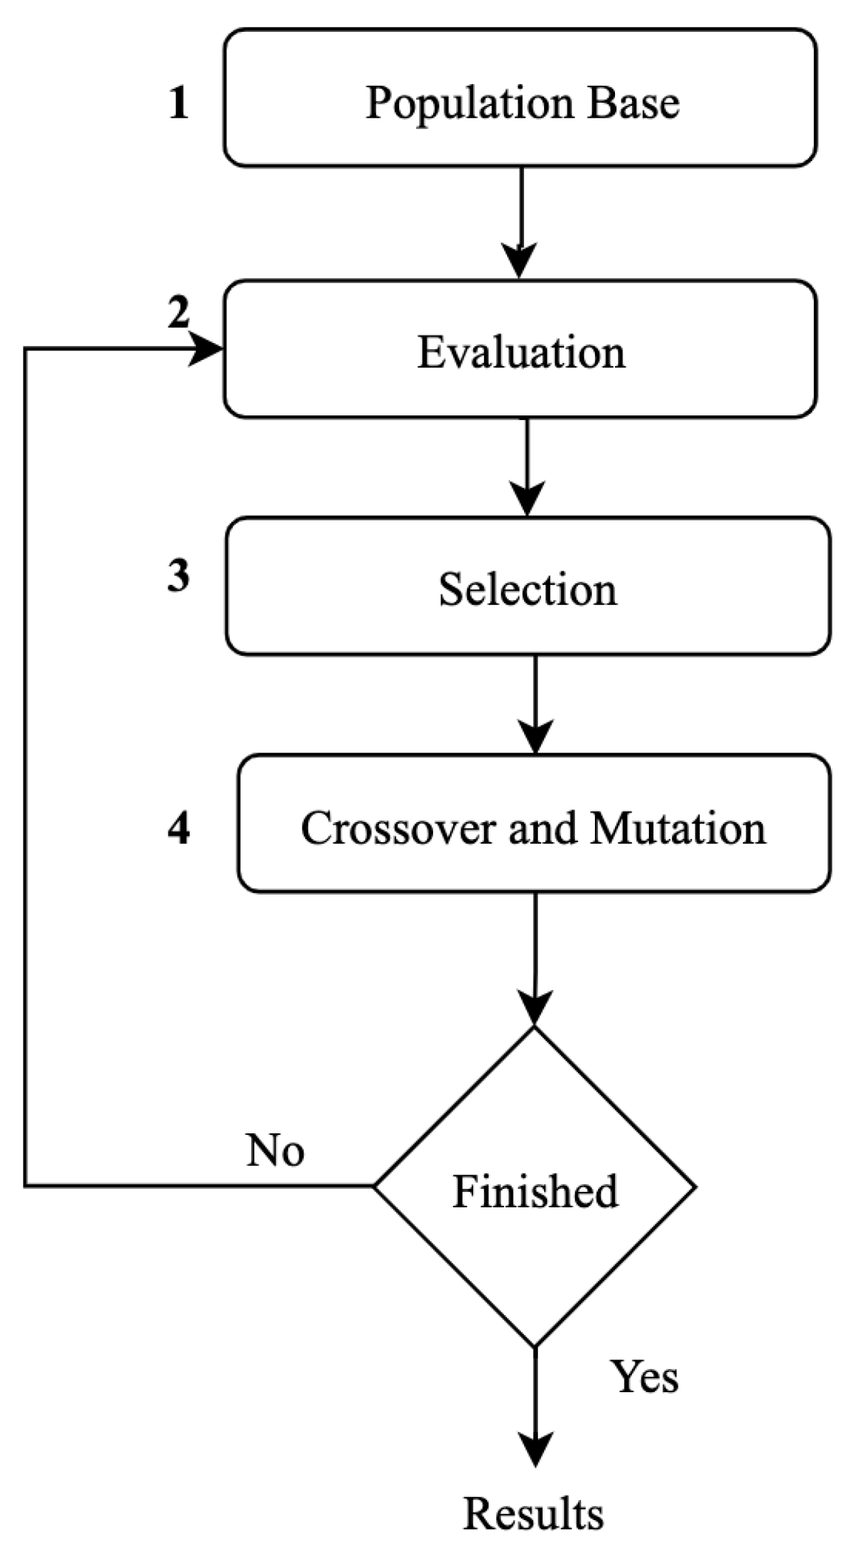
\includegraphics[width = 0.4\linewidth]{pictures/Steps-of-Genetic-Algorithms.png}
\caption{\label{fig:Steps-of-Genetic-Algorithm}A diagram on the steps of a genetic algorithm}
\end{figure}


\subsection{Robo Maze Blast's Default AI Agent}
The game has its own AI agents that will play against the player in the absence of in-real-life adversaries. They share a common behavior and reasoning that can be visualized with the finite-state machine, as shown in 
Figure 3.

%\begin{figure}
%
\includegraphics[width = 1\linewidth]{pictures/bomberman_finite_state_machine 1.png}
%\caption{\label{fig:bomberman_finite_state_machine 1}Finite-state machine of game's AI agent}
%\end{figure}



\section{Fine-tuning agent behaviors with jenetics}


\subsection{Differential Evolution}

\subsection{Agent Behavior}

\subsection{The Reward Metrics}
The fitness function determines which agent behaviors are rewarded, and which are penalized.
\begin{table}[htbp]
\centering

\caption{Agent Reward and Penalty Values}

\begin{tabular}{l|l}
\textbf{Action} & \textbf{Points}  \\
\hline
Movement & +1 (per step) \\
\hline
Place Bomb & +75 (per bomb) \\
\hline
Blow Wall & +150 (per wall) \\
\hline
Kills & +750 (per player) \\
\hline
Death  & -500  \\
\hline
Suicide & -500 \\
\hline
Win without kills & +200  \\
\hline
Win with kills & +1000  \\
\hline
\end{tabular}
\end{table}


\section{Supervised Learning with Jenetics}
\subsection{Introduction}
My objective was to create an AI player using a genetic algorithm (GA) trained on human gameplay data, with an exploration of skill transferability across gaming domains. 
This approach was motivated by competitive gaming frameworks where player strength is quantified through Elo rating systems \cite{elo1978}. 
As an experienced fighting game player, my current Tekken 8 Elo rating stands at \textbf{1940} (profile: \url{https://wank.wavu.wiki/player/3nyHJQr8Gq6Q}, accessed \today). 
While acknowledging that direct skill transfer between a 3D fighting game (Tekken) and a 2D grid-based strategy game (Robo Maze Blast) may be limited, this project tests the hypothesis that:
\begin{center}
    \fbox{\parbox{0.9\linewidth}{
    \textbf{Hypothesis}: Strategic decision-making patterns in high-Elo players exhibit domain-agnostic qualities, such that:
    \begin{equation*}
    \text{Elo}{\text{source}} \geq 1900 \xrightarrow{\text{transfer}} \text{AI}{\text{target}} > \text{AI}_{\text{baseline}} + \Delta
    \end{equation*}
    where $\Delta$ represents measurable skill advantage in Robo Maze Blast.
    }}
\end{center}
%\[
%\text{Mutation}(x) = x + \mathcal{N}(0,\, \sigma^2) \quad \text{where } \sigma = 0.2
%\]
\subsection{Jenetics}
Jenetics is an open-source Java library that provides a genetic Algorithm (GA) framework for solving optimization problems. It abstracts biological evolution principles, such as selection, crossover, and mutation, into re ble software components, enabling users to evolve solutions without implementing a GA from scratch. 
\subsection{Jenetics Framework}
\label{subsec:jenetics}

We selected it for supervised learning because:
\begin{itemize}
    \item \textbf{Prior experience}: We'd successfully used it in previous labs
    \item \textbf{Java compatibility}: Integrated smoothly with our game codebase
    \item \textbf{Rapid adjustments}: Changing parameters takes minutes instead of hours
    \item \textbf{Easy versioning}: Git checkpoints for different \textsf{conf}igurations
\end{itemize}

\textbf{Key Features We Utilized:}
\begin{itemize}
    \item \textbf{Evolutionary engine}: Automatically handles generations and survival mechanics
    \item \textbf{Domain flexibility}: Worked directly with our game strategy optimization
    \item \textbf{Pre-built operators}: 
    \begin{itemize}
        \item Tournament selection (picks winners from random groups)
        \item Gaussian mutation (makes small, smart adjustments)
        \item Single-point crossover (combines parent solutions)
    \end{itemize}
\end{itemize}

\textbf{Agile Implementation:}
The library let us quickly test configurations by reducing parameters:
\begin{itemize}
    \item Population size: 100 $\rightarrow$ 500 
    \item Mutation rate: 0.1 $\rightarrow$ 0.05 
    \item Training generations: 50 $\rightarrow$ 200 
\end{itemize}

This enables an iterative improvement cycles:
\begin{itemize}

    \item [0.] Gather human data
    \item [1.] Train initial AI
    \item [2.] Identify weaknesses
    \item [3.] Adjust parameters
    \item [4.] Retrain (under 30 minutes)
    

\end{itemize}
\noindent\textbf{Reference}: \href{https://jenetics.io/manual/manual-8.2.0.pdf}{Jenetics User Manual} \cite{jenetics2024}.
\subsection{Implementing Gameplay Recording: Code Changes for Data Collection}
\label{subsec:recording}

To train the AI using Jenetics, we first needed good quality gameplay data. The simplest way to get this data was to record what a human player does during a game - both their actions and the game situation at that moment. This required changes to the Player class, which led to creating the new \texttt{RecordablePlayer} class. The main changes are shown in Algorithm~\ref{alg:recording} and include:

\begin{itemize}
	\item \textbf{Recording trigger}: Making the game log actions when players move or place bombs
	\item \textbf{State capture}: Saving player position and bomb status in simple numbers
	\item \textbf{Data export}: Saving all records to a CSV file for AI training
\end{itemize}

\textbf{Example from actual gameplay:}
Imagine this situation during a game:
\begin{itemize}
	\item Player is at position (7, 12) in a 20x20 grid
	\item Player can place a bomb (has bombs available)
	\item There's a bomb nearby above the player
\end{itemize}

The \texttt{RecordablePlayer} would save this information as:\\
\texttt{0.35, 0.60, 1.0, 1.0, -0.4, 5}

\begin{center}
	\begin{tabular}{|l|l|}
		\hline
		\textbf{Value} & \textbf{Meaning} \\ 
		\hline
		0.35 & Player is 35\% across the level (X position) \\ 
		0.60 & Player is 60\% down the level (Y position) \\ 
		1.0 & Bomb available \\ 
		1.0 & Bomb nearby \\ 
		-0.4 & Bomb is above player \\ 
		5 & Player placed a bomb \\ 
		\hline
	\end{tabular}
\end{center}

This simple number format allows the AI to learn from many such records. In the future I would collect a sample trainings data set to train 

\begin{algorithm}[t]
	\caption{RecordablePlayer Modifications}
	\label{alg:recording}
	\DontPrintSemicolon
	\SetKwFunction{GetState}{getStateVector}
	\SetKwFunction{Save}{saveRecordings}
	
	\textbf{Class} RecordablePlayer \textbf{extends} Player\;
	\nl\textbf{New Data:} 
	recordings = [] \;
	isRecording = false \tcp*{Recording on/off switch}
	
	\BlankLine
	\nl\textbf{Key Changes:}\;
	\nl \textbf{move(dx, dy)}:
	super.move(dx, dy)\;
	\If{isRecording}{\textsc{LogMovement}(dx, dy) \tcp*{Records moves}}
	
	\nl \textbf{placeBomb()}:
	super.placeBomb()\;
	\If{isRecording}{\textsc{LogAction}(BOMB) \tcp*{Records bombs}}
	
	\BlankLine
	\nl\textbf{New Methods:}\;
	\nl\textsc{LogMovement}(dx, dy):
	Convert dx/dy to direction\;
	\textsc{LogAction}(direction)\;
	
	\nl\textsc{LogAction}(action):
	state $\leftarrow$ [normX, normY, bombAvail, bombNear]\;
	recordings $\leftarrow$ recordings + (state, action)\;
	
	\nl\textsc{Save}(filename):
	Write all recordings to file\;
\end{algorithm}

\subsection{Data Augmentation for Generating a Training Dataset}
\label{subsec:data_augmentation}

To overcome the limitations of this small sample size, a common challenge in data-intensive tasks like training an AI, we would apply data augmentation techniques. Specifically, we would modify this training data by mirroring gameplay across both the X and Y axes. This simple yet effective method quadruples our dataset, generating new, valid scenarios that maintain the original gameplay logic. As shown in the example below, a leftward movement on the original grid (e.g., player at 0.35) becomes a rightward movement in the mirrored version (0.65), and a downward movement becomes an upward movement (0.40). This process not only increases the quantity of our data but also enhances its diversity, exposing the AI to a broader range of game states and actions.

The use of geometric transformations like mirroring is a well-established method for creating new training samples from a limited dataset \cite{perez2017effectiveness}. This technique is especially useful in supervised learning contexts where the underlying data structure, such as a coordinate system, can be logically transformed without altering the class labels or core relationships within the data.

Looking ahead, we would also explore the possibility of adding additional labels to our data to provide more context. This could include a numerical rating, similar to the Elo system, to grade the quality of a specific action or the player's performance during a session. This would provide the AI with richer context, such as classifying a move as "defensive" or "aggressive," further refining the learning process. This would involve a server-side database to record match outcomes and calculate a lasting Elo rating for different AI player implementations, allowing for a more nuanced and competitive evaluation of fitness over generations.

\subsection{Hypothetical Implementation with Jenetics}
\label{subsec:hypothetical_jenetics}

While not implemented due to time constraints, this section outlines the planned pseudocode structure for the Jenetics-based evolutionary approach. The design reflects best practices in GA configuration with domain-specific adjustments for game AI development.

\label{subsec:hypothetical_jenetics}

\begin{algorithm}[t]
	\caption{Proposed Jenetics Workflow}
	\label{alg:jenetics_hypothetical}
	\DontPrintSemicolon
	\SetKwFunction{Build}{build}
	\SetKwFunction{Collect}{collect}
	
	\textbf{Engine Configuration:}\;
	engine $\leftarrow$ Engine.builder(fitnessFunction, chromosome)\;
	\nl.populationSize(500)          \tcp*{Balanced diversity/computation}\;
	\nl.optimize(Optimize.MAXIMUM)   \tcp*{Maximize fitness score}\;
	\nl.offspringSelector(new TournamentSelector<>(5))\;
	\nl.survivorsSelector(new EliteSelector<>(0.2))\;
	\nl.alterers(\;
	\nl\ \ new Mutator<>(0.12),      \tcp*{Domain-adjusted mutation}\;
	\nl\ \ new SinglePointCrossover<>(0.85)\;
	\nl )\;
	\nl.\Build()\;
	
	\BlankLine
	\textbf{Evolution Execution:}\;
	result $\leftarrow$ engine.stream()\;
	\nl.limit(by(SteadyFitness(15, 50))) \tcp*{Stop when plateau detected}\;
	\nl.peek(stat $\rightarrow$ logGeneration(stat)) \tcp*{Progress tracking}\;
	\nl.\Collect(EvolutionResult.toBestGenotype())\;
\end{algorithm}

\subsubsection{Design Rationale}
The parameter selections balance exploration/exploitation tradeoffs against computational constraints:

\begin{enumerate}
	\item \textbf{Population Size (500)}: 
	Hypothesized to maintain solution diversity while remaining computationally feasible (estimated 35min/generation). Larger than default to counteract premature convergence in complex game state spaces.
	
	\item \textbf{Mutation Rate (0.12)}: 
	Intentionally higher than Jenetics' default (0.01) to prevent behavioral local optima. This would encourage exploration of unconventional strategies (e.g., calculated risk-taking) that might outperform conservative play.
	
	\item \textbf{Steady State Termination}:
	Planned to use fitness plateau detection (15 generations without 0.5\% improvement) rather than fixed generations. This adaptive approach prevents unnecessary computation after convergence.
	
	\item \textbf{Tournament Size (5)}: 
	Maintained at Jenetics' recommendation. Altering this would require simultaneous adjustment of selection pressure metrics - changing multiple interdependent parameters was avoided per \cite{back2000evolutionary}.
	
	\item \textbf{Elite Retention (20\%)}: 
	Conservative preservation of top performers ensures successful tactics propagate while allowing population diversity. This follows standard practice in steady-state evolution \cite{dejong2006evolutionary}.
\end{enumerate}


\subsection{Outlook}
This project encountered several limitations that merit consideration in future work. The primary constraint was the delayed commencement of the implementation phase, attributable to initial uncertainties regarding project specifications and concurrent academic commitments, including a separate laboratory project and examination during the final month. Initiating development 2-3 months earlier upon clarification of assignment parameters would have facilitated more comprehensive implementation.

A critical oversight involved underestimating the integration complexity between the developed AI agent and other project components. Consequently, the planned comparative evaluation against other group members' agents could not be executed. 

Despite these constraints, the project yielded valuable insights regarding data augmentation methodologies, Elo system applications in artificial intelligence, and practical experience with the Jenetics framework. These learnings establish a foundation for future work, which should prioritize agent implementation completion and systematic tournament-based evaluation.
\end{document}
